%-- coding: UTF-8 --
%
\documentclass{llncs}
\usepackage{amsfonts}
\usepackage{amstext}
\usepackage{amsmath}
\usepackage{enumitem}
\usepackage{multirow}
\usepackage{graphicx}
\usepackage[center]{subfigure}
\usepackage{amssymb}
\usepackage{graphicx,amsmath}
\usepackage{subfigure}
\usepackage{algorithm}
\usepackage{algorithmic}
\usepackage{threeparttable}
\renewcommand{\algorithmicrequire}{ \textbf{Input:}}
\renewcommand{\algorithmicensure}{ \textbf{Output:}}
\usepackage{url}
\usepackage{cite}
\usepackage{color}
\usepackage[UTF8]{ctex}
%
\begin{document}

\title{知识表示学习模型的研究}
\author{Anonymous}
\institute{北京航空航天大学计算机学院}
\maketitle

\begin{abstract}

知识图谱是一种可以结构化地表示真实世界中的实体和实体间关系的网络,广泛应用于搜索引擎等领域。近年来,大量开源知识图谱的出现,验证了知识图谱模型在真实世界数据集中的表现。与此同时,专门为知识图谱设计以图论为基础的算法成本越来越高。知识表示学习将知识图谱中的实体和关系转化为低维词向量的形式,来表征其语义联系,使得知识图谱相关研究不必拘束于图的算法。本文将针对近年来具有重要意义的知识表示学习模型进行研究和对比,并介绍知识表示学习领域的其他相关模型。

\keywords{表示学习,知识图谱,知识表示}

\end{abstract}

\section{背景介绍}

\subsection{知识图谱}

知识图谱\cite{DBLP:journals/pieee/Nickel0TG16}是用来表示真实世界中的实体和实体间关系的图结构网络,由节点和边组成,其中节点代表实体,边代表实体之间的关系,通常用三元组 $G=\{E,R,S\}$ 来表示知识图谱,其中 $E$ 为实体的集合, $R$ 为关系的集合, $S$ 是实体-关系-实体的三元组集合,即 $S\subseteq{E×R×E}$ 。此外,一个实体-关系-实体的三元组也可以表示为 $(h,r,t)$ 的格式,其中 $h$ 和 $t$ 分别代表头实体和尾实体, $r$ 表示头实体和尾实体之间的关系。

\subsection{知识图谱数据集}

著名知识图谱开源数据集有 WordNet\cite{Miller:1995:WLD:219717.219748} 、 FreeBase\cite{Bollacker:2008:FCC:1376616.1376746} 、 Wikidata\cite{42240} 和 Yago\cite{suchanek2007yago} 等。其中 WordNet 数据集是由专家构建的词典知识库, FreeBase 数据集则是由志愿者构建的世界知识库,包含人物、地点、分类等信息, Yago 则是一个从半结构化文本中学习出的知识库。知识表示学习的相关算法,大多基于 WordNet 和 FreeBase 进行验证。此外,由于具体应用的特殊性,往往需要将三元组 $S$ 根据实体之间的对应关系分为 $1-1$ 、 $1-n$ 、 $n-1$ 、 $n-n$ 四种。 FB15K 和 WN18 \cite{DBLP:conf/nips/BordesUGWY13}是 FreeBase 和 WordNet 数据集的子集,其数据规模见表\ref{tb:FB15K&WN18}。但在 ConvE 模型\cite{DBLP:conf/aaai/DettmersMS018}中发现,这两个数据集存在严重的测试集泄漏问题,即对于某个训练集中的三元组,反转其头实体和尾实体,就可以在测试集中找到相同的数据。故在此后的研究中,普遍使用去除泄漏数据的 FB15K-237 和 WN18-RR 数据集进行训练、验证和预测。

\begin{table}
	\centering
	\caption{ FB15K 和 WN18 数据集规模}
	\label{tb:FB15K&WN18}
	\begin{threeparttable}
		\begin{tabular}{cccccc}
			\hline
			\textbf{数据集} & \textbf{实体数} & \textbf{关系数} & \textbf{训练集三元组数} & \textbf{验证集三元组数} & \textbf{测试集三元组数} \\ \hline
			WN18 & 40943 & 18 & 141442 & 5000 & 5000 \\
			FB15K & 14951 & 1345 & 483142 & 50000 & 59071 \\ \hline
		\end{tabular}
	\end{threeparttable}
\end{table}

\subsection{知识表示学习的概念}

知识图谱通常以图的形式存储,这种图结构不仅不利于对知识图谱的进一步研究,更需要设计特定的算法进行相应的计算。因此通常将图结构转化为向量的形式,便于更加高效的解决知识图谱领域的关系提取、关系预测、实体预测等问题。

通过向量表示实体的方法通常有两种。在传统方法中,采用独热编码来构建向量。对一个有n个实体数据集,需要对每个实体使用一个n维向量来表示。每个向量中只有 1 维的值为 1 ,其余值均为 0 。这种方法存在明显的问题:随着数据集规模的增加,向量维数过大;又由于向量之间两两正交,不仅无法表示出实体的语义信息,更无法表示实体之间的相似程度。另一种构建词向量的方法则是通过机器学习算法,得到每一个实体的低维稠密向量。对于一个词向量而言,单独拿出一维数值可能毫无意义,但组成词向量后却可以表示出相应实体的语义信息,这就是表示学习。

所谓知识表示学习\cite{DBLP:journals/corr/abs-1812-10901},即对知识库运用表示学习的方法。通过用低维度的稠密向量来表示知识库中的实体或关系,从而进行实体预测\cite{DBLP:journals/tkde/WangMWG17}、实体分类、语义相似性分析等工作。常用的知识表示学习模型可以分为线性模型、神经网络模型、翻译模型等。

\section{模型综述}

见图\ref{fg:resume}。

\begin{figure}
	\centering
	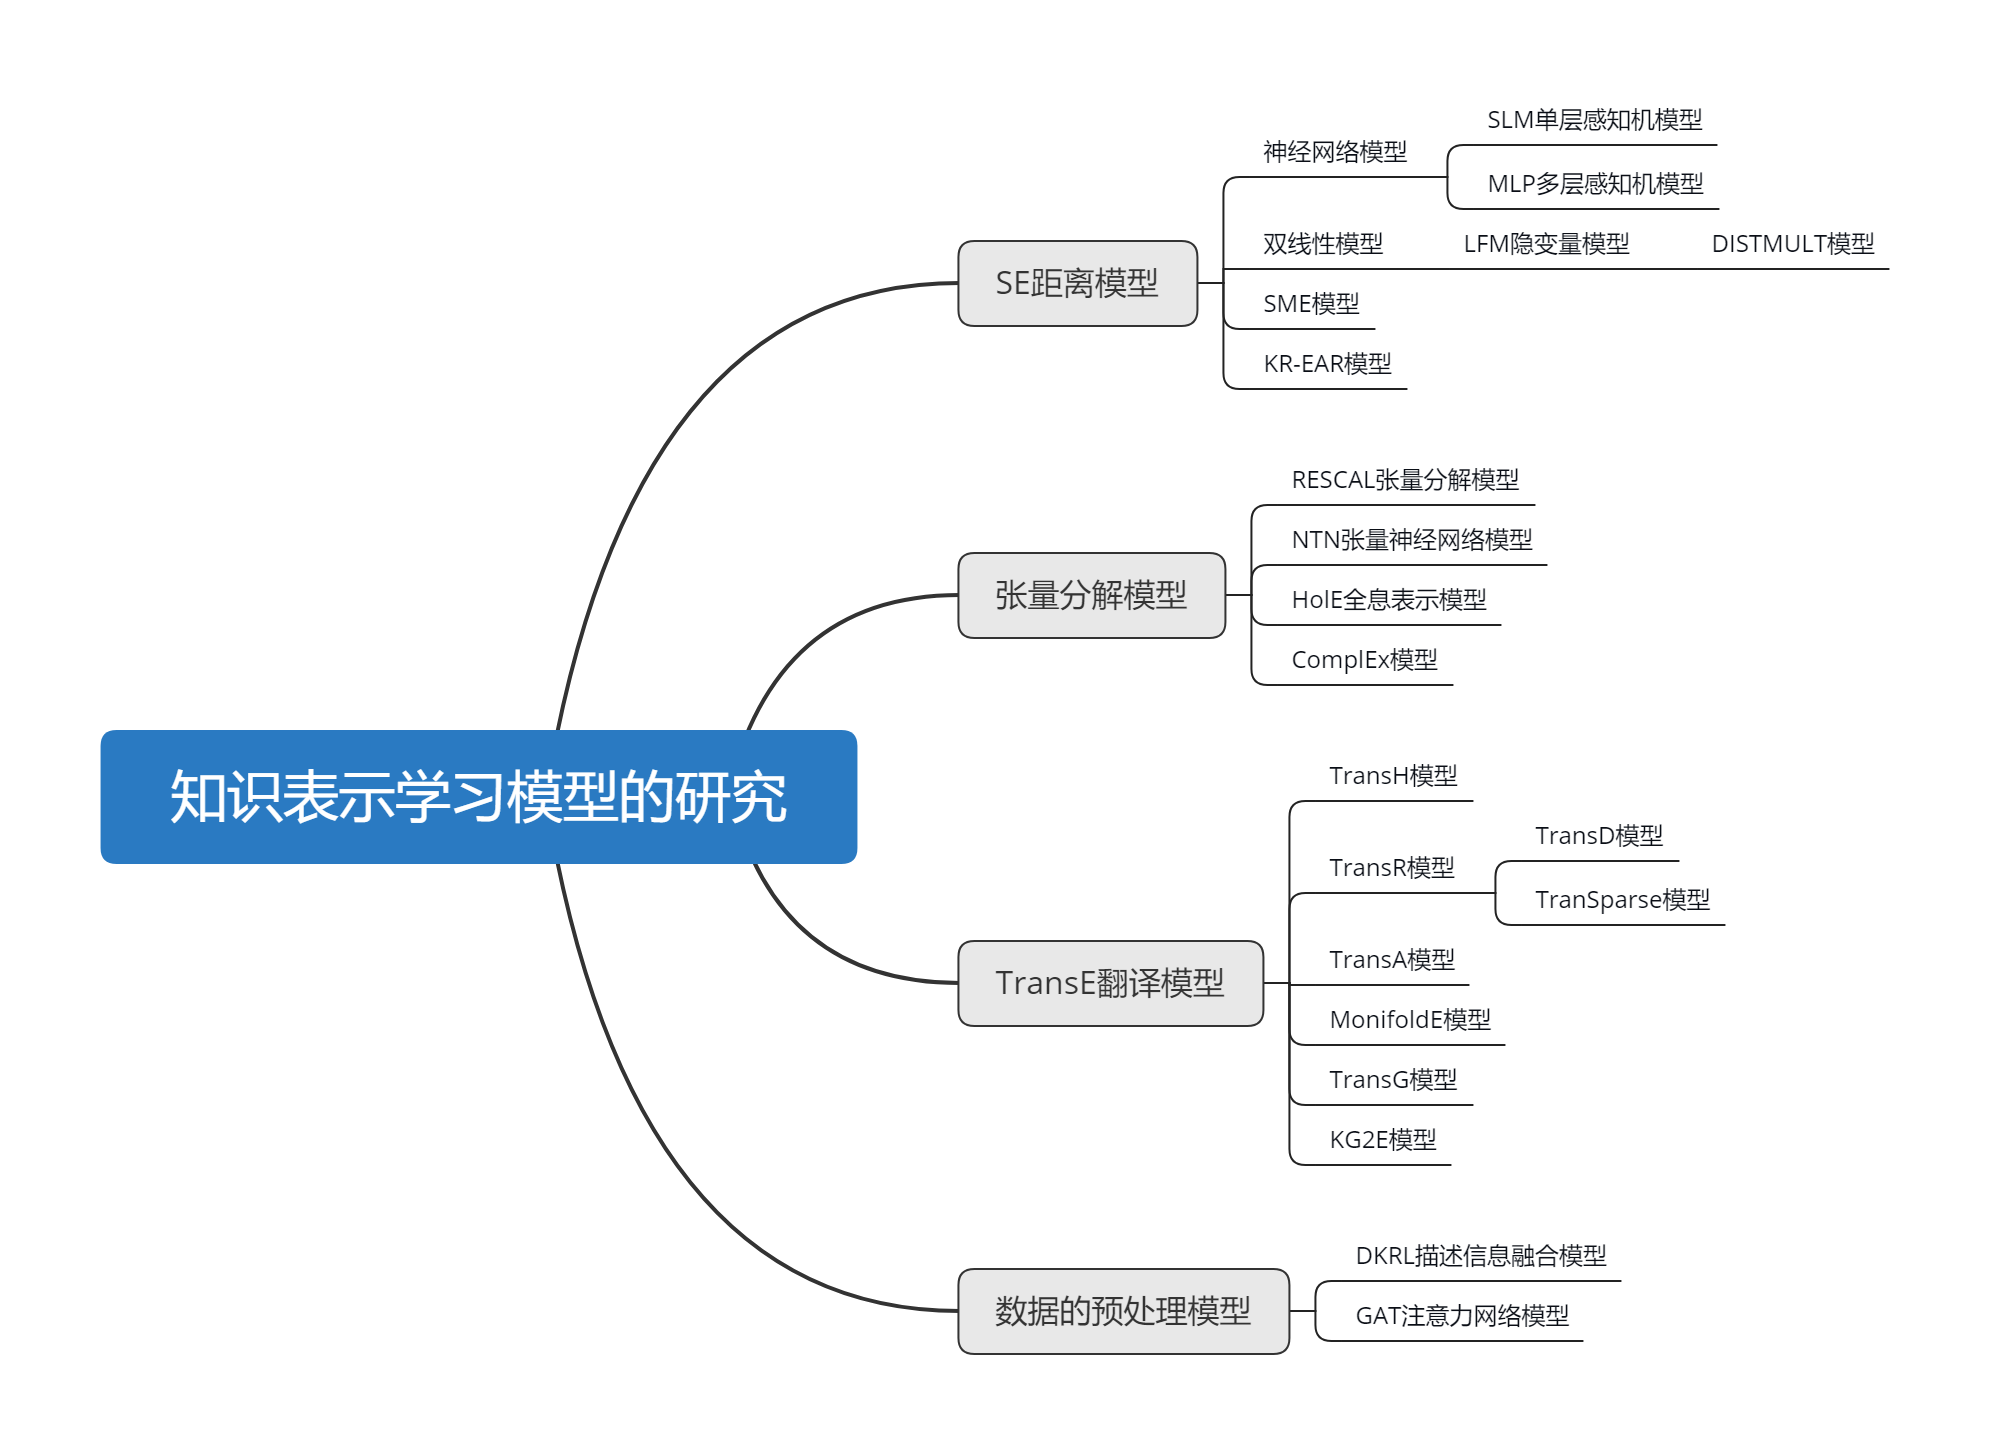
\includegraphics[width=1\columnwidth]{figures/resume.png}
	\caption{模型综述}
	\label{fg:resume}
\end{figure}

\section{知识表示学习模型}

\subsection{距离模型及其扩展模型}

结构表示模型(Structured Embeddings,SE)\cite{DBLP:conf/aaai/BordesWCB11,DBLP:journals/corr/abs-1301-3618}是最经典的线性模型, SE 模型也被称为距离模型。对于知识图谱中的一个头实体-尾实体-关系三元组 $\{E_h, E_t, R_k\}$ , SE 模型通过将第 $x$ 个实体 $E_x$ 表征为一个 $d$ 维(约50维)的词向量 $l_x$ ,将第 $k$ 个关系 $R_k$ 构造成两个 $d×d$ 维的投影矩阵 $W^h_k$ 和 $W^t_k$ ,并定义了如下的损失函数来计算实体之间的语义相关性:
\begin{displaymath}
S_k(E_h,E_t)=||W^h_kl_h-W^t_kl_t||_p
\end{displaymath}
在 SE 模型中,取范数 $p=1$ ,此时损失函数为:
\begin{displaymath}
S_k(E_h,E_t)=\sum_{x=1}^d{S_k(E_h,E_t)_x}
\end{displaymath}
即将头实体和尾实体的词向量分别用一个投影矩阵投影,投影后的距离为投影后得到的向量差按位相加的结果。 SE 模型认为,实体投影后的距离越小,头实体和尾实体的越有可能存在该种关系。因此只需不断迭代使得损失函数最小,求出实体向量 $l$ 和投影矩阵 $W$ 两个参数的最优值。应用在实体预测时,只需通过头实体词向量和两个关系矩阵,即可计算出尾实体映射在该关系平面中的词向量。由于损失函数采用 $L1$ 范数, SE 模型又被称为距离模型。

但使用两个投影矩阵来定义一种关系,很难直观的表征出实体之间的关系。在现实世界中,实体 king 与 queen 之间的关系,应该和实体 man 与 woman 的关系有一定联系。换言之,这两个关系向量应该具有某种相似性。但 SE 模型通过两个投影矩阵来表示一种联系后,很难反映出其中的语义联系。此后出现的单层感知机模型(Single Layer Model,SLM)\cite{DBLP:conf/nips/SocherCMN13}和多层感知机模型(Multi Layer Perceptron,MLP)\cite{DBLP:conf/kdd/0001GHHLMSSZ14},试图在 SE 模型的基础上解决这个问题。 SLM 模型采用了和 SE 模型一样的两个投影矩阵,其评价函数为:
\begin{displaymath}
g(E_h,E_t,R_k)=u_k^Ttanh(W^h_kl_h+W^t_kl_t)
\end{displaymath}
其中 $u_k$ 为关系 $R_k$ 相关的参数。而 MLP 模型可以看作在 SLM 模型的基础上引入多个隐藏层的结果。 SLM 模型和 MLP 模型并非线性模型,而是利用神经网络进行计算,由此带来了挖掘实体和关系之间隐含语义联系的可能性,一定程度上解决了 SE 模型中无法计算实体之间和关系之间的语义联系的问题,但与此同时也大幅提高了参数计算的复杂度,且模型的可解释性较差。

为了进一步解决距离模型中,使用两个投影矩阵无法直观表现关系之间的语义联系的问题,出现了双线性模型。隐变量模型(Latent Factor Model,LFM)\cite{DBLP:conf/nips/JenattonRBO12,NIPS2009_3863}和 DISTMULT 模型\cite{DBLP:journals/corr/YangYHGD14a}就是双线性模型的代表。 LFM 模型可以直观的通过其评价函数来理解:
\begin{displaymath}
g(E_h,E_t,R_k)=l_h^TW_kl_t^T
\end{displaymath}
即头实体向量 $l_h$ 或尾实体向量 $l_t$ 都可以通过一个和关系矩阵的线性变换得到对方。双线性将关系表征为一个二维矩阵,大大简化了距离模型的投影矩阵。而 DISTMULT 模型根据 LFM 模型中和权重乘积的过程,将关系矩阵限制为对角矩阵,即主对角线外的元素值都为0,不仅提升了 LFM 模型的效果,还进一步降低关系矩阵参数的规模。

针对翻译模型中的 TransE 模型\cite{DBLP:conf/nips/BordesUGWY13}中采取了平移的方法,该论文还提出了优化后的 DISTADD 模型\cite{DBLP:journals/corr/YangYHGD14a}, DISTADD 模型和 DISTMULT 模型在实体分类问题上的准确率见表\ref{tb:DISTMULT&DISTADD}。相比之下, DISTMULT 模型的效果更胜一筹。

\begin{table}
	\centering
	\caption{ DISTMULT 模型和 DISTADD 模型在实体分类问题上的准确性}
	\label{tb:DISTMULT&DISTADD}
	\begin{threeparttable}
		\begin{tabular}{ccccccccc}
			\hline
			\textbf{模型} & \multicolumn{4}{c}{\textbf{头实体预测准确率}} & \multicolumn{4}{c}{\textbf{尾实体预测准确率}} \\
			\textbf{} & \textbf{1-1} & \textbf{1-n} & \textbf{n-1} & \textbf{n-n} & \textbf{1-1} & \textbf{1-n} & \textbf{n-1} & \textbf{n-n} \\ \hline
			DISTADD & 70.0 & 76.7 & 21.1 & 53.9 & 68.7 & 17.4 & 83.2 & 57.5 \\
			DISTMULT & 75.5 & 85.1 & 42.9 & 55.2 & 73.7 & 46.7 & 81.0 & 58.8 \\ \hline
		\end{tabular}
	\end{threeparttable}
\end{table}

除此之外,还有双线性的语义匹配能量模型(Semantic Matching Energy,SME)\cite{DBLP:journals/jmlr/BordesGWB12},同样在 SE 模型的基础上尝试构建实体和关系之间的潜在语义联系; KR-EAR 模型\cite{DBLP:conf/ijcai/LinLS16}则通过把关系再细分为属性和关系两种,提高模型在 $1-n$ 和 $n-1$ 等情况的效果。

\subsection{张量分解\cite{harshman1994parafac}模型及其扩展模型}

张量分解模型(RESCAL)\cite{DBLP:conf/icml/NickelTK11,DBLP:conf/www/NickelTK12}又被称为矩阵分解模型,它和 LFM 的思想类似,对第 $k$ 个头实体-关系-尾实体的三元组,定义一个三阶张量:
\begin{displaymath}
\chi_k=AR_kA^T
\end{displaymath}
其中 $A$ 为因子矩阵,是所有实体向量拼接成的矩阵; $R_k$ 为核心矩阵,是关系 $k$ 的参数。参数的求解是通过矩阵分解和交替最小二乘法,图\ref{fg:RESCAL}表示出了 RESCAL 模型的矩阵分解过程。

\begin{figure}
	\centering
	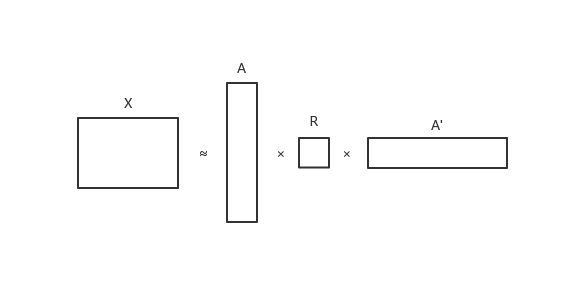
\includegraphics[width=0.8\columnwidth]{figures/RESCAL.png}
	\caption{ RESCAL 模型的矩阵分解}
	\label{fg:RESCAL}
\end{figure}

在 RESCAL 模型中,定义损失函数为:
\begin{displaymath}
\min_{A,R_k}=\frac{1}{2}(\sum_k||\chi_k-AR_kA^T||^2_F)+\frac{1}{2}\lambda(||A||^2_F+\sum_k||R_k||^2_F)
\end{displaymath}
对于每一个可能的三元组,计算其张量 $\chi_k$ 值。在关系预测上,认为张量 $X_k$ 大于阈值则认为关系存在(即认为 $\chi_k=1$ ),小于阈值则认为关系不存在(即认为 $\chi_k=0$ )。 RESCAL 模型也是一个双线性模型,同样也存在参数过大的问题。

张量神经网络模型(Neural Tensor Networks,NTN)\cite{DBLP:conf/nips/SocherCMN13}则是双线性模型和神经网络模型的结合。 NTN 模型是在 SLM 模型的基础上引入实体和关系的三阶双线性张量,如图\ref{fg:NTN}所示。

\begin{figure}
	\centering
	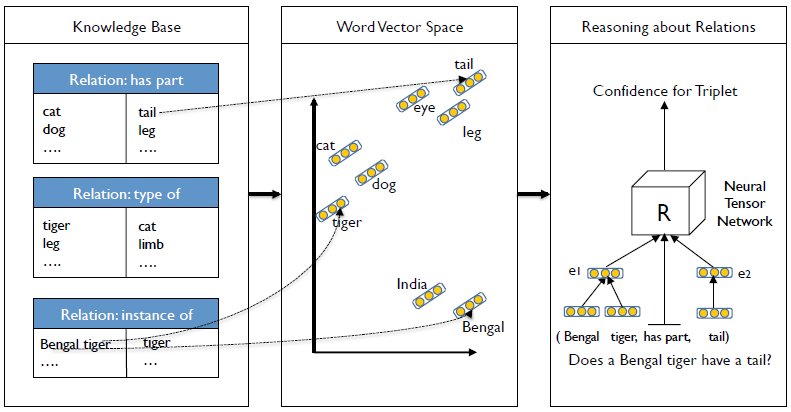
\includegraphics[width=0.8\columnwidth]{figures/NTN.png}
	\caption{ NTN 模型}
	\label{fg:NTN}
\end{figure}
在 NTN 模型中,还对向量进行预训练作为初始值,而不是通常采用的随机生成,这样做的好处是尽可能使用实体和关系的语义信息,尤其是在比较稠密的知识图谱中,对模型效果的提高十分明显。 NTN 模型相比上述模型,对实体和联系的语义信息体现的更好,但 NTN 模型所需要的参数较多,难以在知识图谱较稀疏时发挥作用。

此外,还有使用循环相关(Circular Correlation)代替 RESCAL 模型张量乘积操作的全息表示模型(Holographic Embeddings,HolE)\cite{DBLP:conf/aaai/NickelRP16},该循环相关降低了 RESCAL 模型中的参数维度。 ComplEx 模型\cite{DBLP:conf/icml/TrouillonWRGB16}则同样是在 RESCAL 模型基础上的扩展模型。研究\cite{DBLP:conf/acl/HayashiS17}表明, ComplEx 模型与 HolE 模型在数学上的原理相同。

\subsection{翻译模型及其扩展模型}

\begin{figure}
	\centering
	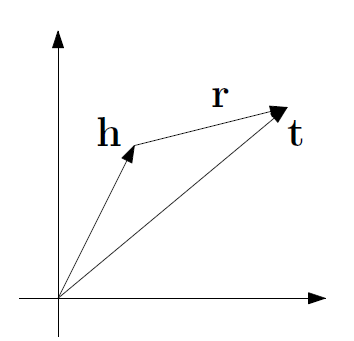
\includegraphics[width=0.5\columnwidth]{figures/TransE.png}
	\caption{ TransE 模型的翻译过程}
	\label{fg:TransE}
\end{figure}

在距离模型及其扩展模型中,关系通常被表征为一个或两个矩阵进行点乘映射。受到 Word2Vec 模型\cite{DBLP:conf/nips/MikolovSCCD13,DBLP:journals/corr/abs-1301-3781}的启发, TransE 模型\cite{DBLP:conf/nips/BordesUGWY13}被称为翻译模型或隐距离模型,它将关系表征为一个向量 $l_r$ 而非矩阵,其“翻译”的过程可以表示为:
\begin{displaymath}
l_t\approx l_h+l_r
\end{displaymath}
即将尾实体的词向量看作头实体按照关系进行平移的结果,图\ref{fg:TransE}直观的反映出了 TransE 模型翻译的过程。相应的, TransE 模型的评分函数为:
\begin{displaymath}
f_r(E_h,E_t)=d(l_h+l_r,l_t)
\end{displaymath}
通过这个平移的过程, TransE 模型 可以很好的表示出实体 king 与 queen 的联系和实体 man 与 woman 的联系的语义相关性。但实验\cite{DBLP:conf/nips/BordesUGWY13}表明, TransE 模型对 $1-n$ 问题的效果并不理想,在实体预测问题上, TransE 模型的准确率见表\ref{tb:TransE}。

\begin{table}
	\centering
	\caption{ TransE 模型在实体预测问题上的准确性}
	\label{tb:TransE}
	\begin{threeparttable}
		\begin{tabular}{ccccccccc}
			\hline
			\textbf{模型} & \multicolumn{4}{c}{\textbf{头实体预测准确率}} & \multicolumn{4}{c}{\textbf{尾实体预测准确率}} \\
			\textbf{} & \textbf{1-1} & \textbf{1-n} & \textbf{n-1} & \textbf{n-n} & \textbf{1-1} & \textbf{1-n} & \textbf{n-1} & \textbf{n-n} \\ \hline
			SME & 30.9 & 69.6 & 19.9 & 38.6 & 28.2 & 13.1 & 76.0 & 41.8\\
			TransE & 43.7 & 65.7 & 18.2 & 47.2 & 43.7 & 19.7 & 66.7 & 50.0 \\ \hline
		\end{tabular}
	\end{threeparttable}
\end{table}

对于 $1-n$ 问题,如“苹果公司的创始人有谁”应该有多个尾实体符合。但经过 TransE 模型训练后,由 $l_h+l_r$ 得到的尾实体向量相同,即多个创始人有着相同的词向量,这显然与显示不符。但由于 TransE 模型可以通过向量直接建立语义联系,且参数大幅减少,性能提升较大,逐渐成为了相当经典的模型。后续许多扩展模型都是根据 TransE 翻译模型进行的进一步改进。

针对 TransE 模型中在 $1-n$ 、 $n-1$ 和 $n-n$ 问题上的缺陷,提出了 TransH 模型\cite{DBLP:conf/aaai/WangZFC14}。不同于 TransE 模型中,简单的将头实体词向量根据关系向量平移, TransH 模型采用了向量投影的方法,如图\ref{fg:TransH}所示。

\begin{figure}
	\centering
	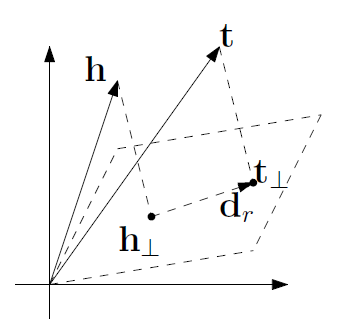
\includegraphics[width=0.5\columnwidth]{figures/TransH.png}
	\caption{ TransH 模型的翻译过程}
	\label{fg:TransH}
\end{figure}

在 TransH 模型中,认为在不同的关系中的实体应该有不同的表示。 TransH 模型通过定义投影矩阵 $W_r$ ,将头实体向量 $l_h$ 和尾实体向量 $l_t$ 投影到投影平面,得到 $l_{h\perp}$ 和 $l_{t\perp}$ 向量。此后再使用 TransE 模型的方法进行翻译:
\begin{displaymath}
l_{t\perp}\approx l_{h\perp}+l_r
\end{displaymath}
而投影的过程,可以表示为:
\begin{displaymath}
	\begin{split}{}
	l_{h\perp}&=l_h-W_r^ThW_r \\
	l_{t\perp}&=l_t-W_r^TtW_r
	\end{split}
\end{displaymath}
通过投影操作, TransH 模型实际只使用了实体词向量的一个分量,避免出现 TransE 模型在非 $1-1$ 情况下得到相同尾实体的问题,更好的区分了。 TransR 模型\cite{DBLP:conf/aaai/LinLSLZ15}同样认为,实体有多种不同的表示。但与 TransH 模型不同的是,在 TransR 模型中,实体的不同方面不仅仅统一空间的向量分解,而是应当对不同的关系,建立不同的关系空间进行投影。投影的过程见图\ref{fg:TransR},具体投影公式为:
\begin{displaymath}
	\begin{split}
	l_{hr}&=l_hW_r \\
	l_{tr}&=l_tW_r
	\end{split}
\end{displaymath}

\begin{figure}
	\centering
	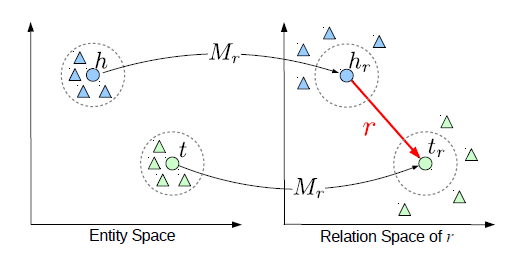
\includegraphics[width=0.5\columnwidth]{figures/TransR.png}
	\caption{ TransR 投影过程}
	\label{fg:TransR}
\end{figure}

此外,还有改善 TransR 模型映射规则的 TransD 模型\cite{DBLP:conf/er/XiongHD18},使用将 TransR 模型中的稠密矩阵更换为稀疏矩阵的 TranSparse 模型\cite{DBLP:conf/aaai/JiLH016},更改距离度量方式为马氏距离的 TransA 模型\cite{DBLP:journals/corr/0005HHZ15a},使用流形代替传统 $L_1$ 或 $L_2$ 距离的 ManifoldE 模型\cite{DBLP:conf/ijcai/0005HZ16},增加高斯混合的 TransG 模型\cite{DBLP:journals/corr/0005HHZ15},使用高斯分布重新描述实体和关系的 KG2E 模型\cite{DBLP:conf/cikm/HeLJ015}等,都是对 TransE 模型的扩展。

\section{知识表示学习数据的预处理模型}

\subsection{多源数据融合}

知识图谱如 FreeBase 的数据不仅包含简单的三元组,对于每一个实体,包括实体描述、实体分类等信息没有被知识表示学习算法所利用。为了融合实体和关系的描述信息,提出了 DKRL 模型\cite{DBLP:conf/aaai/XieLJLS16}。在 DKRL 模型中,使用了 连续词袋神经网络模型(Continuous Bag-of-words Encoder,CBOW)\cite{DBLP:journals/corr/abs-1301-3781}和卷积神经网络模型(Convolutional Neural Network,CNN)\cite{DBLP:conf/icml/CollobertW08}。 CBOW模型通过将实体描述的词进行拼接后,预测其中心词,见图\ref{fg:CBOW}。 DKRL 模型最终得到的是融合了实体和关系描述信息的词向量,以及每个实体相关的中心词,可代替其他知识表示学习模型的随机初始化过程。

\begin{figure}
	\centering
	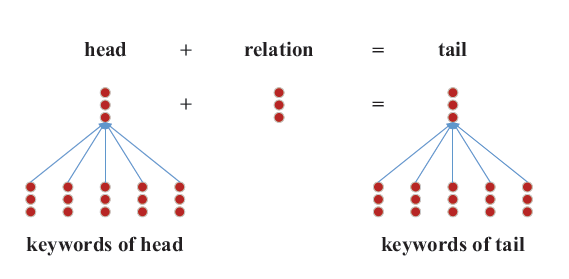
\includegraphics[width=0.8\columnwidth]{figures/CBOW.png}
	\caption{ CBOW 过程}
	\label{fg:CBOW}
\end{figure}

\subsection{实体分类预处理}

GAT 模型\cite{DBLP:conf/iclr/VelickovicCCRLB18}提出了一种基于注意力机制的节点分类。注意力机制(Attention)\cite{DBLP:journals/corr/BahdanauCB14}中,每个节点可以和使用其他节点的特征,为其分配不同的权值,作为自己的特征。在 GAT 模型中使用的是通过masked self-attention机制,即只计算与该实体相邻的实体特征,见图\ref{fg:GAT}。
\begin{figure}
	\centering
	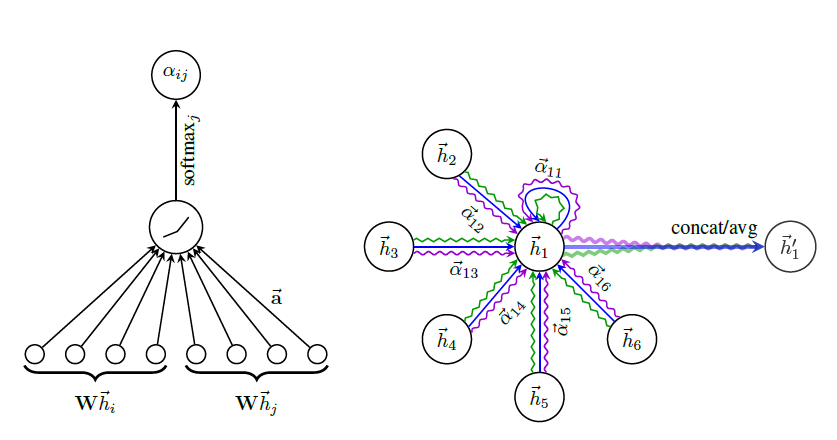
\includegraphics[width=0.8\columnwidth]{figures/GAT.png}
	\caption{ GAT 模型}
	\label{fg:GAT}
\end{figure}
 GAT 模型的输出为对实体词向量分类后的词向量。相比 GCN 模型\cite{DBLP:conf/iclr/KipfW17,DBLP:conf/nips/DefferrardBV16}, GAT 模型更加高效, attention 机制中每个节点的重要程度可以不同,使得 GAT 模型有更强的表示能力。

\section{结论}

通过研究和比对知识表示学习模型的发展过程和最新进展,可以发现,越来越多的模型侧重于发现实体之间、实体和关系之间的隐含语义联系,以提升预测的准确性。大多数模型都是在几个经典模型(如距离模型、翻译模型)的基础上,针对其出现的问题和不足进行改进。目前,知识表示学习模型大多还存在着诸如参数过多、对稀疏知识图谱表现差、难以挖掘隐含语义联系、可解释性差等诸多问题。但随着知识图谱的应用越来越广泛,知识表示模型的改进并不会停止,期待未来越来越多的模型会解决已知的问题,拓宽知识图谱的应用领域。

\bibliographystyle{splncs03}
%\bibliographystyle{unsrt}
\bibliography{reference}
	
\end{document}
